\documentclass{article}

\usepackage{graphicx}
\usepackage{tikz}
\usepackage{tikzsymbols}
\usetikzlibrary{calc,patterns,shapes.geometric}
\pagestyle{empty}
\usepackage[margin=0pt]{geometry}
\geometry{papersize={14in,12in}}

\def\centerarc[#1](#2)(#3:#4:#5){\draw[#1] ($(#2)+({#5*cos(#3)},{#5*sin(#3)})$) arc (#3:#4:#5);}

\begin{document}
	\begin{figure}
		\centering
		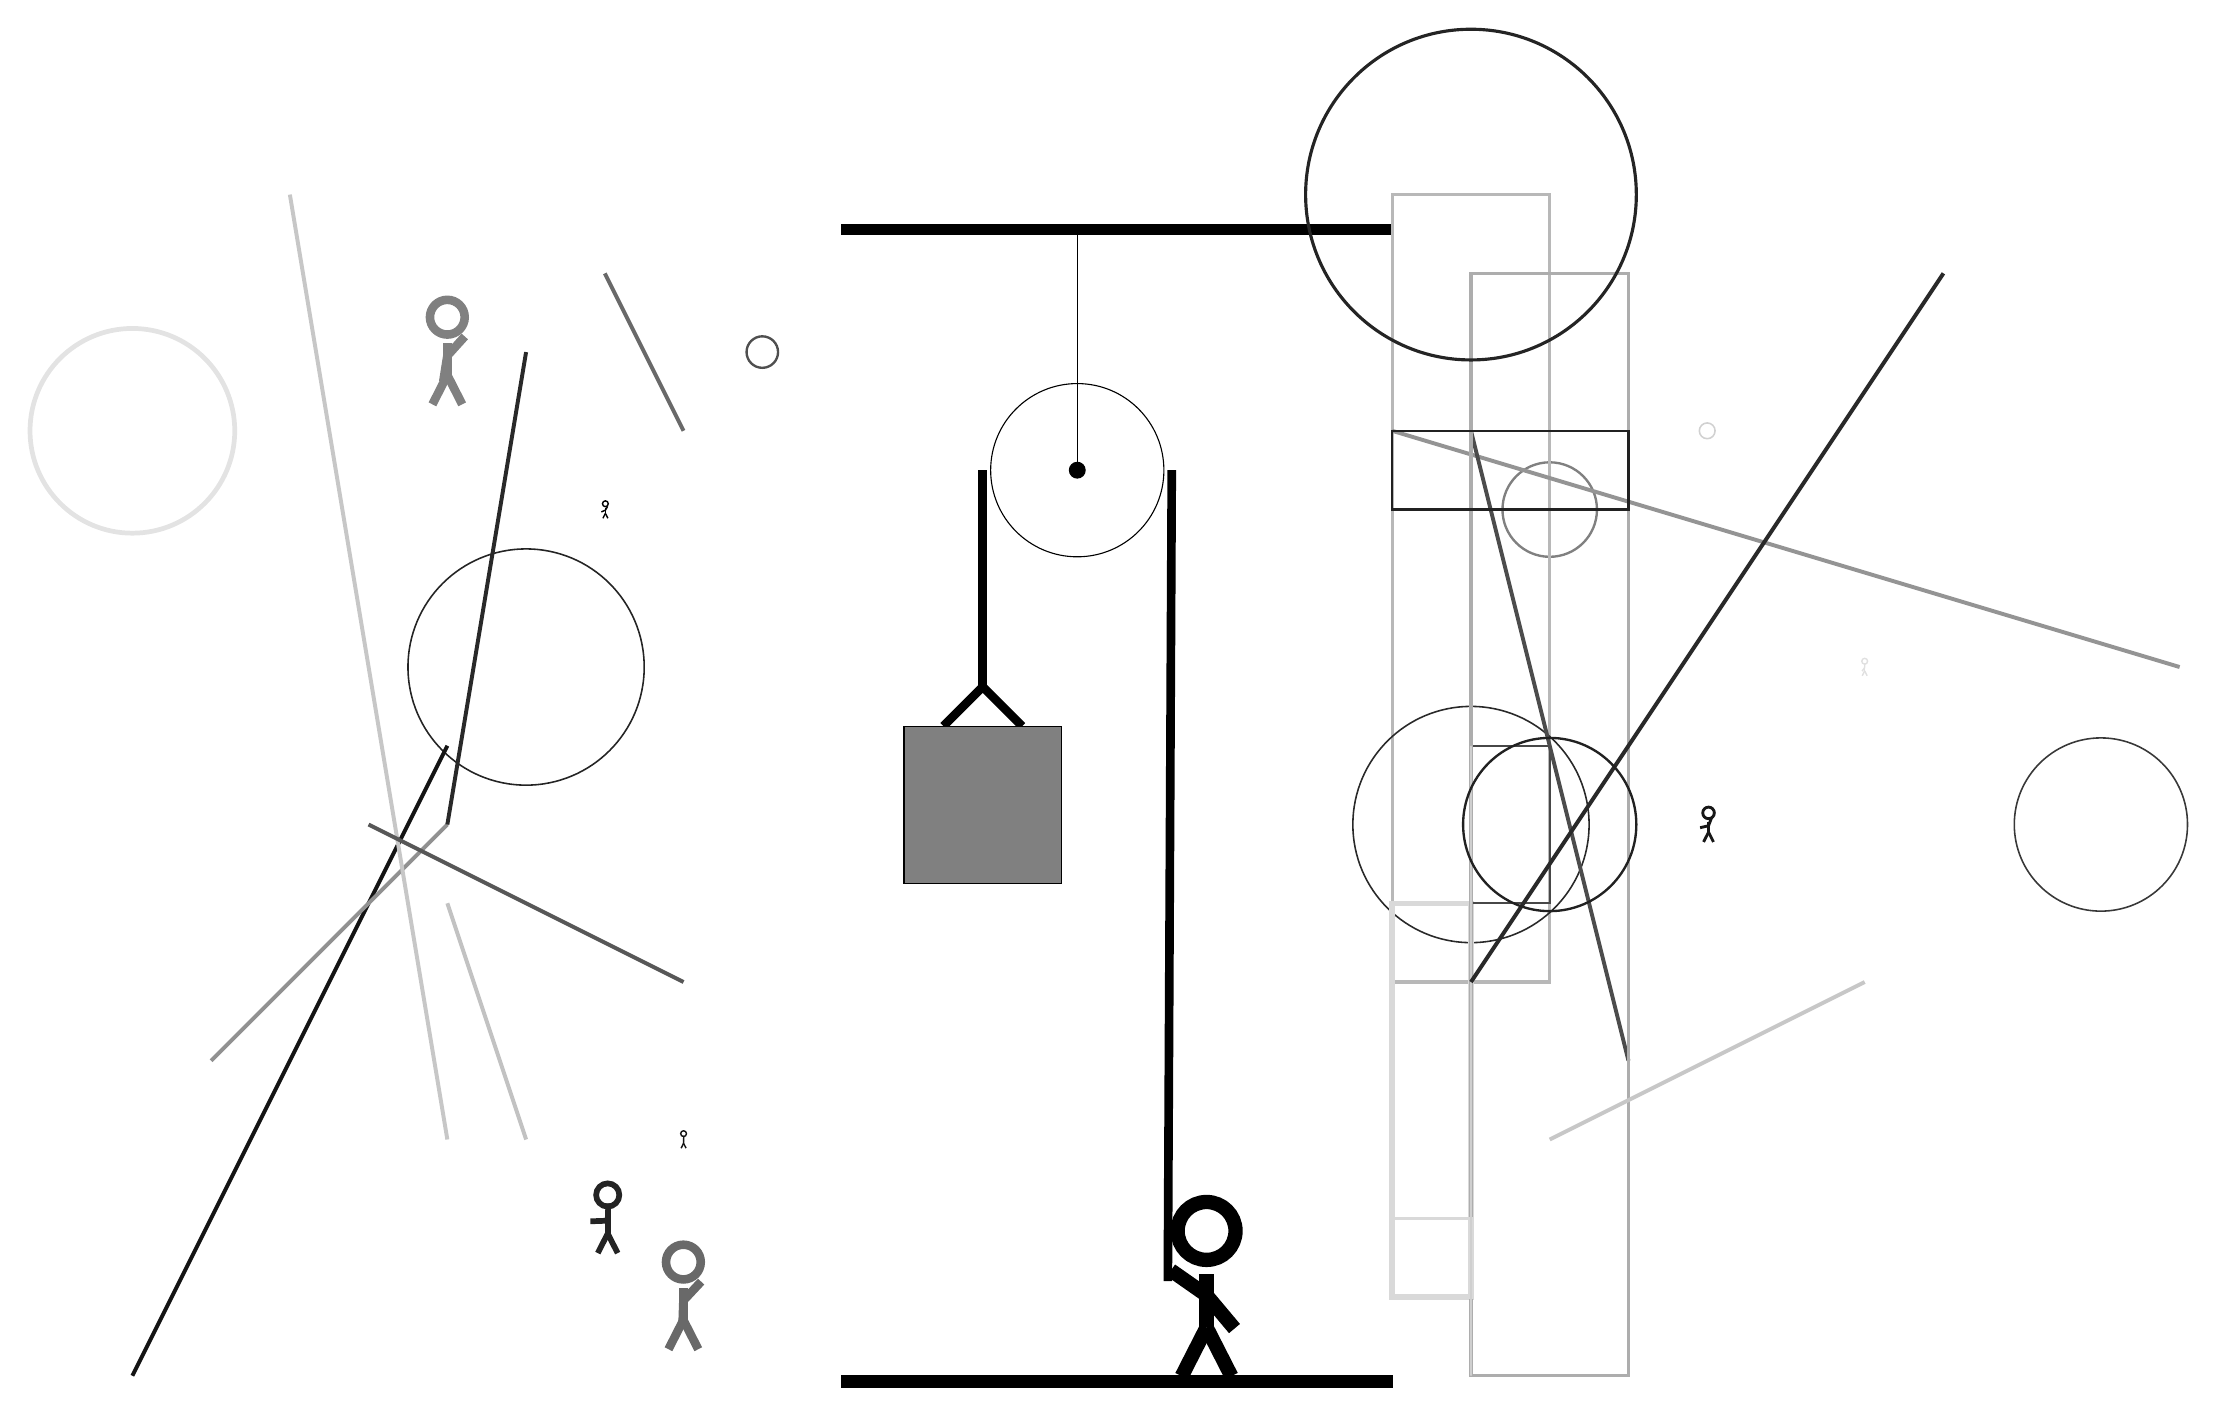
\begin{tikzpicture}
			%%%%% START %%%%%
			
			\draw[fill=black] (-2, 11.5) rectangle (5, 11.625);
			
			\draw (1, 8.5) circle (1.1);
			\draw[fill=black] (1, 8.5) circle (0.1);
			\draw (1, 11.5) -- (1, 8.5);
			
			\draw [line width=0.3mm, color=black!50](7, 8) circle (0.6);
			
			\draw[line width=0.4mm, color=black!28] (5, 2) rectangle (7, 12);
			\draw [line width=0.2mm, color=black!78](14, 4) circle (1.1);
			\draw[line width=0.5mm, color=black!42](5, 9) -- (15, 6);
			\draw [line width=0.2mm, color=black!84](6, 4) circle (1.5);
			
			\draw[line width=0.7mm, color=black!15] (6, -2) rectangle (5, 3);
			\node[line width=0.7mm, color=black!59] at (-4, -2) {\Strichmaxerl[6][88][47]};
			\draw [line width=0.3mm, color=black!69](-3, 10) circle (0.2);
			\node[line width=0.2mm, color=black!86] at (-5, -1) {\Strichmaxerl[4][2][88]};
			
			\draw [line width=0.2mm, color=black!86](-6, 6) circle (1.5);
			\node[line width=0.3mm, color=black!100] at (-5, 8) {\Strichmaxerl[1][23][59]};
			\draw [line width=0.7mm, color=black!72](-4, -1) circle (0.0);
			\draw[line width=0.5mm, color=black!92](-7, 5) -- (-11, -3);
			\draw[line width=0.3mm, color=black!72] (7, 5) rectangle (6, 3);
			\draw[line width=0.5mm, color=black!43](-7, 4) -- (-10, 1);
			\draw[line width=0.5mm, color=black!70](6, 9) -- (8, 1);
			
			\draw[line width=0.4mm, color=black!32] (6, -3) rectangle (8, 11);
			\draw[line width=0.5mm, color=black!24](-6, 0) -- (-7, 3);
			\draw[line width=0.4mm, color=black!15] (5, -1) rectangle (6, -2);
			\node[line width=0.4mm, color=black!92] at (-4, 0) {\Strichmaxerl[1][89][86]};
			\node[line width=0.2mm, color=black!12] at (11, 6) {\Strichmaxerl[1][53][88]};
			\draw[line width=0.2mm, color=black!19] (6, -3) rectangle (6, 5);
			\draw[line width=0.3mm, color=black!87] (5, 8) rectangle (8, 9);
			\draw [line width=0.4mm, color=black!86](6, 12) circle (2.1);
			\node[line width=0.4mm, color=black!91] at (9, 4) {\Strichmaxerl[2][13][69]};
			\draw[line width=0.5mm, color=black!22](7, 0) -- (11, 2);
			\draw[line width=0.5mm, color=black!22](-7, 0) -- (-9, 12);
			\draw[line width=0.5mm, color=black!66](-4, 2) -- (-8, 4);
			
			\draw [line width=0.2mm, color=black!18](9, 9) circle (0.1);
			\draw[line width=0.5mm, color=black!84](-7, 4) -- (-6, 10);
			\draw[line width=0.5mm, color=black!84](6, 2) -- (12, 11);
			
			\draw [line width=0.3mm, color=black!87](7, 4) circle (1.1);
			\draw[line width=0.5mm, color=black!59](-4, 9) -- (-5, 11);
			\node[line width=0.2mm, color=black!50] at (-7, 10) {\Strichmaxerl[6][81][48]};
			\draw [line width=0.6mm, color=black!11](-11, 9) circle (1.3);
			
			\draw[line width=1.1mm] (-0.7, 5.25) -- (-0.2, 5.75) -- (0.3, 5.25);
			\draw[fill=black!50] (-1.2, 5.25) rectangle (0.8, 3.25);
			
			\draw[line width=1.1mm] (-0.2, 8.5) -- (-0.2, 5.75);
			\centerarc[line width=1.1mm](1, 8.5)(0:180:1.2000000000000002);
			\draw[line width=1.1mm](2.2, 8.5) -- (2.15, -1.8);
			
			\node at (2.6, -1.9) {\Strichmaxerl[10][-35][-50]};
			
			\draw[fill=black] (-2, -3) rectangle (5, -3.15);
			
			%%%%% END %%%%%
		\end{tikzpicture}
	\end{figure}	
\end{document}